\documentclass[a4paper,UTF8]{article}
\usepackage{ctex}
\usepackage[margin=1.25in]{geometry}
\usepackage{color}
\usepackage{graphicx}
\usepackage{amssymb}
\usepackage{amsmath}
\usepackage{amsthm}
\usepackage{soul, color, xcolor}
\usepackage{bm}
\usepackage{tcolorbox}
\usepackage{hyperref}
\numberwithin{equation}{section}
%\usepackage[thmmarks, amsmath, thref]{ntheorem}
\theoremstyle{definition}
\newtheorem*{solution}{Solution}
\newtheorem*{prove}{Proof}
\usepackage{multirow}
\usepackage{diagbox}
\usepackage{float}
\usepackage{mathtools}
\def \X {\mathbf{X}}
\def \Z {\mathbf{Z}}
\def \W {\mathbf{W}}
\def \A {\mathbf{A}}
\def \K {\mathbf{K}}
\def \B {\mathbf{B}}
\def \C {\mathbf{C}}
\def \Q {\mathbf{Q}}
\def \S {\mathbf{S}}
\def \P {\mathbf{P}}
\def \Diag {\textbf{$\Lambda$}}
\def \w {\hat{\boldsymbol{w}}}
\def \y {\boldsymbol{y}}
\def \x {\boldsymbol{x}}
\def \z {\mathbf{z}}
\def \b {\mathbf{b}}
\def \by {\Bar{y}}
\def \H {\mathbf{H}}
\def \I {\mathbf{I}}
\setlength{\parindent}{0pt}
%--

%--
\begin{document}
\title{机器学习导论\ 习题五}
\author{学号, 姓名, \href{mailto:邮箱}{邮箱}}
\maketitle
\section*{作业提交注意事项}
\begin{tcolorbox}
	\begin{enumerate}
    \item[1.] 作业所需的LaTeX及Python环境配置要求请参考: \href{https://www.lamda.nju.edu.cn/ML2024Spring/supplemantary/environment.pdf}{[Link]};
		\item[2.] 请在LaTeX模板中第一页填写个人的学号、姓名、邮箱;
		\item[3.] 本次作业需提交的文件与对应的命名方式为:
            \begin{enumerate}
                \item [(a)] 作答后的LaTeX代码 --- \texttt{HW5.tex};
                \item [(b)] 由(a)编译得到的PDF文件 --- \texttt{HW5.pdf};
                \item [(c)] 第四题 AdaBoost 代码 --- \texttt{AdaBoost.py};
                \item [(d)] 第四题 Random Forest 代码 --- \texttt{RandomForest.py};
                \item [(e)] 第四题绘图代码 --- \texttt{main.py}.
            \end{enumerate}
            请将以上文件{\color{red}\textbf{打包为~学号\hspace{0em}\_\hspace{0em}姓名.zip}} (例如 221300001\hspace{0em}\_\hspace{0em}张三.zip) 后提交;
		\item[3.] 若多次提交作业, 则在命名~.zip 文件时加上版本号, 例如 221300001\_\hspace{0em}张三\hspace{0em}\_v1.zip” (批改时以版本号最高的文件为准);
		\item[4.] 本次作业提交截止时间为 {\color{red}\textbf{ 6 月 14 日23:59:59}}. 未按照要求提交作业, 提交作业格式不正确, {\color{red}\textbf{作业命名不规范}}, 将会被扣除部分作业分数; 除特殊原因 (如因病缓交, 需出示医院假条) 逾期未交作业, 本次作业记 0 分; {\color{red}\textbf{如发现抄袭, 抄袭和被抄袭双方成绩全部取消}};
        \item[5.] 学习过程中, 允许参考 ChatGPT 等生成式语言模型的生成结果, 但必须在可信的信息源处核实信息的真实性; {\color{red}\textbf{不允许直接使用模型的生成结果作为作业的回答内容}}, 否则将视为作业非本人完成并取消成绩;
		\item[6.] 本次作业提交地址为 \href{https://box.nju.edu.cn/u/d/06ad1043a3dd4ecebc80/}{[Link]}, 请大家预留时间提前上交, 以防在临近截止日期时, 因网络等原因无法按时提交作业.
	\end{enumerate}
\end{tcolorbox}
\newpage


  \section{[25pts] Naive Bayesian}
朴素贝叶斯是一种经典的生成式模型. 请仔细学习《机器学习》第七章 7.3 节, 并完成下题. 

\begin{table}[H]
\label{tab:data1}
\centering
\begin{tabular}{c|*{15}{c}}
    \hline
   & 1 & 2 & 3 & 4 & 5 & 6 & 7 & 8 & 9 & 10 & 11 & 12 & 13 & 14 & 15 \\
  \hline
  $X^{(1)}$ & 1 & 1 & 1 & 2 & 2 & 2 & 2 & 3 & 3 & 3 & 3 & 3 & 3 & 3 & 3 \\
  $X^{(2)}$ & S & M & L & S & M & L & S & M & L & S & M & L & S & M & L \\
  $Y$ & 1 & 1 & -1 & 1 & -1 & -1 & 1 & 1 & 1 & -1 & 1 & 1 & -1 & 1 & 1 \\
  \hline
\end{tabular}
\end{table}       
\begin{enumerate}
    \item[(1)] \textbf{[10pts]} 使用表~\ref{tab:data1}的数据训练朴素贝叶斯模型. 给定新的输入 $x = (2, M)^\top$, 试计算 $\mathbb{P}(x=1)$ 以及 $\mathbb{P}(x=-1)$, 并判断该样本应当被分为哪一类.
    \item[(2)] \textbf{[10pts]} 若使用 “拉普拉斯修正” 训练模型, 对于新输入 $x = (2, M)^\top$, 试计算此时的 $\mathbb{P}_\lambda (x=1)$ 以及 $\mathbb{P}_\lambda (x=-1)$, 并判断此时该样本应当被分为哪一类. 
    \item[(3)] \textbf{[5pts]} 根据以上结果, 试讨论在朴素贝叶斯模型中, 使用 “拉普拉斯修正” 带来的好处与影响.
\end{enumerate}

 
\begin{solution}
    此处用于写解答 (中英文均可)
    ~\\
\end{solution}


\newpage
\section{[25pts] Nearest Neighbor}
假设数据集$\{\mathbf{x}_1,...,\mathbf{x}_n\}$是从一个以$\mathbf{0}$为中心的$p$维单位球中独立均匀采样而得到的$n$个样本点. $p$维单位球可以表示为:
\begin{equation}
	B = \{\mathbf{x}: \lVert \mathbf{x} \rVert^2 \leq 1\} \subset \mathbb{R}^p.
\end{equation}
其中,$\lVert \mathbf{x} \rVert= \sqrt{\langle\mathbf{x}, \mathbf{x}\rangle}$,$\langle\mathbf{x}, \mathbf{x}\rangle$是$\mathbb{R}^p$空间中向量的内积.
在本题中,我们将探究原点$O$与其最近邻($1$-NN)的距离$d^*$,以及$d^*$与$p$之间的关系. $O$与其$1$-NN之间的距离定义为:
\begin{equation}
d^* \coloneqq \min_{1\leq i \leq n} \lVert \mathbf{x}_i \rVert,
\end{equation}
不难发现$d^*$是一个随机变量,因为$\mathbf{x}_i$是随机产生的.
\begin{enumerate}
\item[(1)] \textbf{[5pts]} 当$p=1$且$t\in [0,1]$时,请计算$\mathbb{P}(d^*\leq t)$,即随机变量$d^*$的累积分布函数(Cumulative Distribution Function, $\mathbf{CDF}$).
\item[(2)] \textbf{[7pts]} 请写出$d^*$的$\mathbf{CDF}$的一般公式,即当$p\in\{1,2,3,...\}$时$d^*$对应的取值. 

(\textbf{Hint:} 半径为$r$的$p$维球体积是:$V_p(r)=\frac{(r\sqrt{\pi})^p}{\Gamma(p/2+1)}$, 
	其中,$\Gamma(1/2)=\sqrt{\pi}$,$\Gamma(1)=1$,且有$\Gamma(x+1)=x\Gamma(x)$对所有的$x>0$成立;并且对于$n\in\mathbb{N}^*$,有$\Gamma(n+1)=n!$.)
\item[(3)] \textbf{[8pts]} 请求解随机变量$d^*$的中位数,  \textcolor{blue}{请写成关于$n$和$p$的函数}.

(\textbf{Hint:} 即使得$\mathbb{P}(d^*\leq t)=1/2$成立时的$t$值)
\item[(4)] \textbf{[5pts]} 结合以上问题, 谈谈你关于$n$和$p$以及它们对$1$-NN的性能影响的理解.
\end{enumerate}

\begin{solution}
    此处用于写解答 (中英文均可)
    ~\\
\end{solution}

\newpage

\section{[25pts] K-means and EM Algorithm}
EM (Expectation-Maximization) 算法是存在 “未观测” 变量的情况下估计参数隐变量的利器. 
请仔细阅读《机器学习》第九章以及第七章7.6节, 回答以下问题.

\subsection{[10pts] K-means and GMM}
在《机器学习》9.4.3节中, 我们在聚类问题下推导了高斯混合模型(GMM)的EM算法, 即高斯混合聚类. 沿用该小节中的记号, 我们考虑一种简化后的高斯混合模型, 
其中高斯混合分布共由$k$个混合成分组成, 且每个混合成分拥有相同的协方差矩阵$\Sigma_i = \varepsilon^2 \mathbf{I}, i \in [k]$.
假设$\exists \delta > 0$使得对于选择各个混合成分的概率有$\alpha_i \geq \delta, \forall i \in [k]$, 并且在高斯混合聚类的迭代过程中始终有
$\|\x_i - \mu_k\|^2 \neq \|\x_i - \mu_{k^\prime}\|^2 \text{ for } \forall i \in [n], k \neq k^\prime$ 成立.

\begin{itemize}
    \item[(1)] \textbf{[10pts]} 请证明: 随着$\varepsilon^2 \to 0$, 高斯混合聚类中的$\mathbf{E}$步会收敛至$k$均值聚类算法中簇划分的更新规则, 即每个样本点仅指派给一个高斯成分. 由此可见, $k$均值聚类算法是高斯混合聚类的一种特例.
\end{itemize}

\subsection{[15pts] EM for Survival Analysis}
生存分析 (Survival Analysis) 是一类重要的研究问题. 考虑如下图~\ref{fig:data}所示场景, 医院收集了病人接受治疗后的生存时间数据, 并在时刻 $T=a$ 停止了收集. 假设病人接受治疗后的生存时间服从正态分布分布 $\mathcal{N}(\theta, 1)$. 若一共有 $m$ 个病人参与实验, 其中在 $T=a$ 之前死亡的人数为 $n$, 收集其生存时间数据为 $\X = \{x_1, \cdots, x_n, \underbrace{a, \cdots, a}_{m-n \text{ 个 } a}\}$, 希望使用 EM 算法估计 $\theta$. 
\vskip -0.15in
\begin{figure}[h]
        \centering
        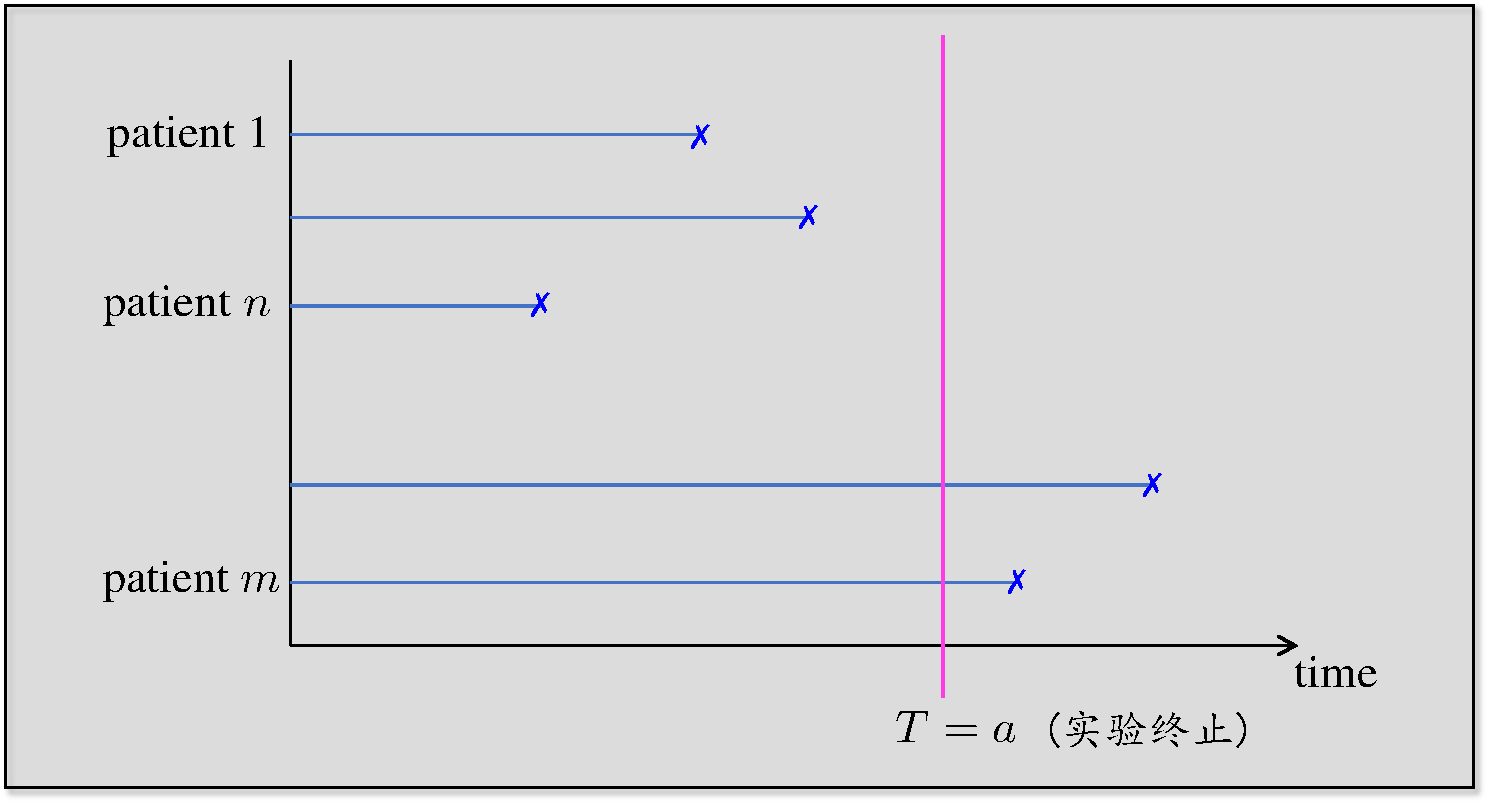
\includegraphics[width=.7\textwidth]{survival-analysis.pdf}
        \vskip -0.1in
        \caption{右删失 (right censored) 生存分析数据示意}
        \label{fig:data}
    \end{figure}
    
\begin{itemize}
    \item[(2)] \textbf{[10pts]} $\mathbf{E}$步: (\textbf{Hint:} observed dataset $\X$ implies that $z_i\geq a, i=1, \cdots, m-n$.)
    \begin{itemize}
    \item[(a)] \textbf{[2pts]} 记 $\mathcal{N}(0, 1)$ 的 CDF 为 $\Phi(\cdot)$, 直接写出似然函数 $L(\X; \theta)$. 
    \item[(b)] \textbf{[3pts]} 记未观测生存时间数据为 $\Z=\{z_1, \cdots, z_{m-n}\}$. 试求对数似然函数 $\log L(\X, \Z; \theta)$. 
    \item[(c)] \textbf{[5pts]} 试求 $f(z_i\mid \X, \theta_t)$, 并依此写出 $Q(\theta\mid \theta_t)$.
    \end{itemize}
    \item[(3)] \textbf{[5pts]} $\mathbf{M}$步: 记 $\mathcal{N}(0, 1)$ 的 PDF 为 $\phi(\cdot)$, 试求 $\theta$ 的更新公式(\textcolor{blue}{使用 $\phi(\cdot)$, $\Phi(\cdot)$ 表示}).
\end{itemize}

\begin{solution}
    此处用于写解答 (中英文均可)
    ~\\
\end{solution}


\newpage
\section{[25pts] Ensemble Methods}

在本题中, 我们尝试使用 AdaBoost 与 Random Forest 这两种经典的集成学习的方法进行分类任务. 本次实验使用的数据集为 UCI 二分类数据集 Adult (Census Income).\\关于编程题的详细说明, 请参考: \href{https://www.lamda.nju.edu.cn/ML2024Spring/homework/HW5/guide.pdf}{编程题指南.pdf}.


\begin{enumerate}
    \item [(1)] \textbf{[10pts]} 请参考《机器学习》中对 AdaBoost 与 Random Forest 的介绍, 使用决策树作为基分类器, 实现 AdaBoost 分类器与 Random Forest 分类器.
    \item [(2)] \textbf{[10pts]} 请基于上述实现, 通过 5-折交叉验证, 探究基学习器数量对集成效果的影响.\\\textcolor{blue}{(请在报告中附上绘制的折线图, 并简要论述分类器数量对分类效果的影响.)}
    \item [(3)] \textbf{[5pts]} 请分别汇报最优超参数 (即: 基学习器数量) 下, 两种模型在测试集上的 AUC 指标 \textcolor{blue}{(结果保留三位小数)}.
\end{enumerate}

\begin{solution}
    此处用于写解答(中英文均可)
    ~\\
\end{solution}

\newpage

\section*{Acknowledgments}
允许与其他同样未完成作业的同学讨论作业的内容, 但需在此注明并加以致谢; 如在作业过程中, 参考了互联网上的资料, 且对完成作业有帮助的, 亦需注明并致谢.

\end{document}